\documentclass[aps,pra,reprint,amsmath,amssymb,nofootinbib,floatfix]{revtex4-2}
\usepackage[UTF8,fontset=fandol,scheme=plain]{ctex}
\usepackage{amsthm,mathtools}
\usepackage{microtype,graphicx,booktabs}
\usepackage[colorlinks=true,linkcolor=blue,citecolor=blue,urlcolor=blue]{hyperref}
\hypersetup{pdfauthor={Tingyu Zhang and Yan Cen},pdftitle={时间齐次量子比特动力学的尖锐重置误差边界}}
\newtheoremstyle{aps}{\topsep}{\topsep}{\normalfont}{\parindent}{\itshape}{.}{ }{}
\theoremstyle{aps}
\newtheorem{theorem}{定理}
\newtheorem{lemma}[theorem]{引理}
\newtheorem{proposition}[theorem]{命题}
\newtheorem{corollary}[theorem]{推论}
\DeclareMathOperator{\tr}{tr}
\DeclareMathOperator{\diag}{diag}
\newcommand{\Q}{\mathcal Q_2}
\newcommand{\Diss}{\mathcal D}
\newcommand{\eps}{\epsilon}
\newcommand{\pos}[1]{\left[#1\right]_+}
\newcommand{\ket}[1]{|#1\rangle}
\newcommand{\bra}[1]{\langle#1|}
\newcommand{\proj}[1]{|#1\rangle\langle#1|}
\renewcommand{\proofname}{证明}
\renewcommand{\abstractname}{摘要}
\renewcommand{\refname}{参考文献}
\renewcommand{\appendixname}{附录}
\renewcommand{\figurename}{图}
\renewcommand{\acknowledgmentsname}{致谢}
\begin{document}
\title{时间齐次量子比特动力学的尖锐重置误差边界}
\author{Tingyu Zhang}
\email{23300190021@m.fudan.edu.cn}
\author{Yan Cen}
\email[通讯作者：]{cenyan@fudan.edu.cn}
\affiliation{Department of Physics, Fudan University, Shanghai, China}

\begin{abstract}
使用时间无关 Lindblad 生成元重置量子比特时，需要同时考虑从一个输入中移除非目标态布居，以及对目标输入造成的扰动。定量刻画二者的权衡，需要在与同一制备和测量基相容的所有生成元上优化。对于向 $\ket1$ 的重置，记 $a=P(0|0)$、$\eps=P(0|1)$。本文确定了固定实际扰动 $\eps$ 时的最大布居排序反转量 $G(\eps)=\max(\eps-a)$。当 $\eps\downarrow0$ 时，在所有量子比特 Lindblad 生成元产生的转移概率及其闭包中，$G(\eps)\sim(4/e)\eps/\log(1/\eps)$。若生成元存在一个在制备—测量基中对角的稳态，则尖锐规律为 $G_{\rm diag}(\eps)\sim(64/e^2)\eps/\log^2(1/\eps)$。显式的单跳跃算符动力学可以达到这两条规律。两种尺度分别源于倾斜稳态本征基中的直接相干读出，以及相干性向布居的反馈。对任何达到不受限首项规律的有限生成元序列，稳态相干性的模平方均与 $\eps$ 渐近相等，而纯度缺陷为 $o(\eps)$。这些结果定量揭示了稳态相干性在自治重置中的作用，并为齐次量子嵌入给出尖锐端点约束。
\end{abstract}
\maketitle

\section{引言}\label{sec:setting}

自治重置利用固定的开放系统动力学制备目标态。对于量子比特，同一个生成元既要从一个基态输入中移除非目标态布居，也要限制对目标输入的扰动。判断这两个条件概率能否同时由时间无关量子 Markov 演化产生，是一个齐次量子嵌入问题。

Shahbeigi 等人研究了随机矩阵的齐次量子嵌入，给出了解析排除区域和数值边界候选 \cite{Shahbeigi2024}。其四参数单跳跃算符族为本文的构造提供了直接基础。该族的数值表现尚未确立它在全部生成元中的最优性。本文的贡献是确定完整生成元类的尖锐端点边界，同时给出存在对角稳态的生成元所具有的不同边界，以及达到首项最优值所必需的稳态结构。

相关相干机制已有研究基础。量子固定点可达范围可以超出经典布居可达范围 \cite{KorzekwaLostaglio2021}；当相干性将信息返回布居时，量子动力学的经典约化也可能失去 $P$ 可分性 \cite{Benatti2024}。下文定量确定\emph{单个时间无关生成元}在重置附近允许的最大布居反转。第 \ref{sec:model} 节定义模型与误差权衡，第 \ref{sec:results} 节陈述尖锐界及稳态约束，第 \ref{sec:mechanisms} 节和第 \ref{sec:universal} 节分别给出达到边界的动力学与普适上界，第 \ref{sec:discussion} 节讨论物理意义、与已有工作的关系及开放问题，第 \ref{sec:conclusions} 节总结主要结论。



\section{模型}\label{sec:model}

将量子比特分别制备为 $\ket0$ 或 $\ket1$，施加相同演化、持续相同时长，再在同一基中测量。在向 $\ket1$ 重置的附近，将列随机概率转移表写为

\begin{equation}\label{eq:table}
 T(a,1-\eps)=\begin{pmatrix}a&\eps\\1-a&1-\eps\end{pmatrix}.
\end{equation}
这里，$a$ 是需要重置的输入所产生的非目标态输出布居，$\eps$ 是施加于目标输入的扰动。二者之差为

\begin{equation}\label{eq:det}
 q:=a-\eps=\det T.
\end{equation}
对于非目标态布居为 $r$ 的对角输入，由线性性可得
\begin{equation}\label{eq:population-order}
 \rho_r=r\proj0+(1-r)\proj1,\qquad
 P_0(r)=\eps+(a-\eps)r.
\end{equation}
因此，$q<0$ 意味着初始非目标态布居更多的输入，最终的非目标态布居反而更少。本文研究当动力学由一个固定的量子比特 Lindblad 生成元产生时，这种反转最多能有多大。

固定\emph{实际测得的} $\eps$，就选定了齐次嵌入区域的一个截面。对于已实现的反转量 $\Delta=\eps-a>0$，所有对角输入中的最坏布居误差仍为 $\eps$，而两种基态输入的等权误差为 $\eps-\Delta/2$。因此，本文关注以输入为条件的布居数据。若只规定允许误差 $\eps\le\delta$，并允许任意时长和速率，向 $\ket1$ 的普通阻尼已能在 $\eps=0$ 时趋近完美重置。这两个测得的概率也没有指定信道对相干输入的响应。



本文考虑所有时间无关的量子比特 GKSL 生成元 \cite{GKS1976,Lindblad1976}

\begin{equation}\label{eq:gksl}
 \begin{gathered}
 \mathcal L(\rho)=-i[H,\rho]+\sum_\mu\Diss[J_\mu](\rho),\\
 \Diss[J](\rho)=J\rho J^\dagger-\tfrac12\{J^\dagger J,\rho\},
 \end{gathered}
\end{equation}
其作用空间为 $\mathbb C^2$，哈密顿量为厄米矩阵，跳跃算符为有限多个、矩阵元均有限的矩阵。系统没有辅助能级，制备和测量所用的基始终固定。速率、持续时间及哈密顿量强度均不受限制。

将每个转移表 $T(a,1-\eps)$ 与坐标对 $(a,1-\eps)$ 对应。记 $\mathcal Q_2^{\rm fin}$ 为有限时长 $t\ge0$ 下由 $e^{t\mathcal L}$ 得到的转移表集合，并令

\begin{equation}\label{eq:closure}
 \Q=\overline{\mathcal Q_2^{\rm fin}}\subset[0,1]^2.
\end{equation}
这采用了文献 \cite{Shahbeigi2024} 中允许任意精度逼近的约定：每个逼近项的参数均有限，但无需共同的速率或时间上界。通过缩放 $H\mapsto tH$、$J_\mu\mapsto\sqrt tJ_\mu$，可以将观测时间固定为一，同时保留奇异参数序列。

固定实际扰动后，定义

\begin{equation}\label{eq:G}
 G(\eps)=\max\{\eps-a:(a,1-\eps)\in\Q\}.
\end{equation}
由于 $\Q$ 是紧集，最大值存在。其截面非空：经典弛豫至布居为 $\eps$ 的状态，在闭包中给出 $a=\eps$。特别地，$0\le G(\eps)\le\eps$。

记 $\mathcal Q_{\rm diag}$ 为有限实现的概率闭包，其中每个生成元都至少存在一个在制备—测量基中对角的稳态。该类允许瞬态相干性及布居—相干耦合，既不要求稳态唯一，也不要求保持所有对角态。在式 \eqref{eq:G} 中以 $\mathcal Q_{\rm diag}$ 替换 $\Q$，定义 $G_{\rm diag}$。

\section{重置误差界}\label{sec:results}\label{sec:diagonal}

在完美重置附近，上述两类动力学具有不同的渐近边界。

\begin{theorem}[自治重置的尖锐规律]\label{thm:main}
对于完整的时间无关量子比特 GKSL 概率闭包，有
\begin{equation}\label{eq:main}
 \lim_{\eps\downarrow0}\frac{\log(1/\eps)}{\eps}G(\eps)=\frac4e.
\end{equation}
等价地，重置区域的下边界满足
\begin{equation}\label{eq:boundary}
 \min\{a:(a,1-\eps)\in\Q\}
 =\eps\left[1-\frac{4/e+o(1)}{\log(1/\eps)}\right].
\end{equation}
\end{theorem}

\begin{theorem}[对角稳态规律]\label{thm:diagonal}
这一受限类具有如下尖锐端点渐近式：
\begin{equation}\label{eq:diagonal-law}
 G_{\rm diag}(\eps)=\left(\frac{64}{e^2}+o(1)\right)
 \frac\eps{\log^2(1/\eps)}.
\end{equation}
\end{theorem}

两条规律都表明，最优边界上有 $a/\eps\to1$：两种输入对应的条件误差在首项上一致，较小的差值 $\eps-a$ 则刻画量子布居反转。该反转量的相对大小在完美重置极限下趋于零。

这两条规律位于经典动力学与含时量子控制之间：
\begin{equation}\label{eq:three}
 \begin{aligned}
 G_{\rm cl}(\eps)&=0,&
 G_{\rm diag}(\eps)&\sim\frac{64}{e^2}\frac{\eps}{\log^2(1/\eps)},\\
 G(\eps)&\sim\frac4e\frac{\eps}{\log(1/\eps)},&
 G_{\rm td}(\eps)&=\eps.
 \end{aligned}
\end{equation}
这里，$G_{\rm cl}$ 和 $G_{\rm td}$ 分别对应经典两态动力学与含时量子比特 GKSL 控制，采用相同的固定误差优化及概率闭包约定。即使允许经典速率随时间变化，仍有
\[
q(t)=\exp[-\int_0^t(k_{01}(s)+k_{10}(s))\,ds]\ge0.
\]
含时量子比特 GKSL 控制可以实现所有两态随机转移表 \cite{KorzekwaLostaglio2021}。这些比较采用相同的系统维数、基和概率任务。

达到不受限的首项最优值，还要求实现序列中每个生成元的所有稳态具有特定结构。对于满足 $a\le\eps$ 且误差足够小的实现，每个稳态都可在其本征基中写为

\begin{equation}\label{eq:stationary}
 \begin{gathered}
 \rho_*=\nu\proj e+(1-\nu)\proj g,\\
 0\le\nu<\tfrac12,\qquad p=|\langle0|g\rangle|^2.
 \end{gathered}
\end{equation}
\begin{corollary}[稳态误差预算的饱和]\label{cor:saturation}
考虑一列参数逐项有限的量子比特 GKSL 实现，其实际误差为 $a_n,\eps_n$，其中 $\eps_n\downarrow0$，且
\begin{equation}\label{eq:saturation}
 \frac{\log(1/\eps_n)}{\eps_n}(\eps_n-a_n)\longrightarrow\frac4e.
\end{equation}
对每个充分大的 $n$，任取一个稳态，并按式 \eqref{eq:stationary} 定义 $\nu_n,p_n$。则
\begin{equation}\label{eq:rigidity}
 \frac{\nu_n}{\eps_n}\longrightarrow0,
 \qquad\frac{p_n}{\eps_n}\longrightarrow1.
\end{equation}
\end{corollary}
在固定测量基中，这给出
\begin{equation}\label{eq:coherence-purity}
 \begin{gathered}
 \left|\bra0\rho_{*,n}\ket1\right|^2
 =(1-2\nu_n)^2p_n(1-p_n)\sim\eps_n,\\
 1-\tr(\rho_{*,n}^2)=2\nu_n(1-\nu_n)=o(\eps_n).
 \end{gathered}
\end{equation}
稳态相干性趋于零，但其模平方占据了布居误差预算的首项。混合度在该预算中所占的比例必须趋于零。这是有限实现序列的必要结构，并未为抽象闭包点指定生成元。证明见第 \ref{sec:universal} 节。

\begin{equation}\label{eq:ratio}
 \frac{G_{\rm diag}(\eps)}{G(\eps)}
 \sim\frac{16}{e\log(1/\eps)}\longrightarrow0.
\end{equation}
因此，任意满足
$\liminf\log(1/\eps)(\eps-a)/\eps>0$
的有限生成元序列，从某一项起都不存在测量基中的对角稳态：否则相应子列满足定理 \ref{thm:diagonal}，其缩放增益必趋于零。要达到不受限首项尺度的渐近非零比例，稳态相干性是必要的；单凭瞬态相干性仍能实现较小的尺度。



\section{渐近最优构造}\label{sec:mechanisms}

两种渐近界可由不同的布居—相干耦合路径达到。图 \ref{fig:gain-comparison} 在同一尺度上比较了具有相同\emph{实际} $\eps$ 的显式实现。这些构造给出下界；在有限误差下，它们的大小关系未必等同于各自优化类别的大小关系。

\begin{figure}[tbp]
 \centering
 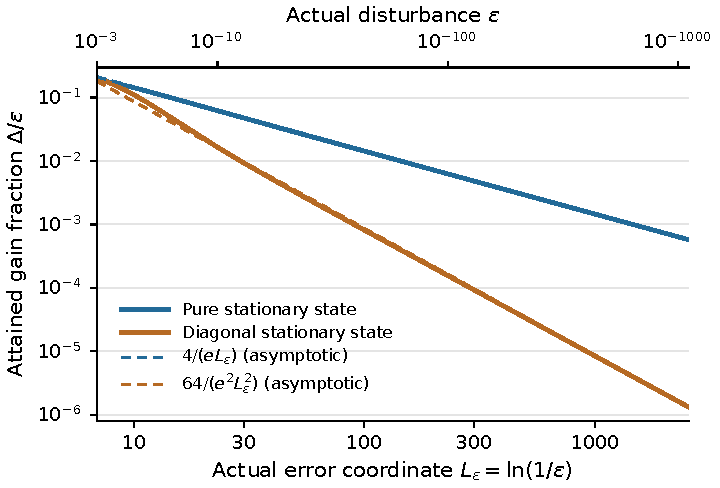
\includegraphics[width=\columnwidth]{reset_gain_comparison.pdf}
 \caption{相同实际扰动 $\eps=P(0|1)$ 下的布居排序反转，以 $\Delta/\eps$ 表示，其中 $\Delta=\eps-a$。实线分别为倾斜纯态构造［式 \eqref{eq:familyparams}--\eqref{eq:familyjump}］和对角态构造［式 \eqref{eq:diag-jump}--\eqref{eq:diag-xstar}］。虚线为其首项规律 $4/(eL_\eps)$ 和 $64/(e^2L_\eps^2)$，其中 $L_\eps=\log(1/\eps)$。实线给出相应最优反转量的可实现下界。在 $\eps=10^{-3}$ 时，对角构造高于图示纯态构造；定理 \ref{thm:main} 和 \ref{thm:diagonal} 的层次关系渐近成立。}
 \label{fig:gain-comparison}
\end{figure}

\subsection{倾斜纯稳态}

对满足 $p=|\langle0|g\rangle|^2$ 的稳态本征向量，采用读出系数
\begin{equation}\label{eq:vw}
 \begin{gathered}
 v=1-2p,\qquad w=2\sqrt{p(1-p)},\\
 V=v^2,\quad W=w^2,\quad R=vw.
 \end{gathered}
\end{equation}
令 $L\to\infty$，并定义
\begin{equation}\label{eq:familyparams}
 p=e^{-L},\qquad A=L+\log L+1-\log4,\qquad B=A/L.
\end{equation}
取正交归一态
\begin{equation}\label{eq:familybasis}
 \ket g=\sqrt p\ket0+\sqrt{1-p}\ket1,\qquad
 \ket e=\sqrt{1-p}\ket0-\sqrt p\ket1,
\end{equation}
在有序基 $(e,g)$ 中，取单个跳跃算符且不加哈密顿量：
\begin{equation}\label{eq:familyjump}
 J=\begin{pmatrix}-\sqrt B&0\\\sqrt A&0\end{pmatrix},\qquad H=0.
\end{equation}
对于每个充分大的有限 $L$，该生成元均以 $\proj g$ 为稳态。对状态 $\rho$，定义布居 $n=\bra e\rho\ket e$ 和相干项 $z=\bra e\rho\ket g$。测得的布居为 $P_0=p+vn+w\operatorname{Re}z$，其动力学满足
\begin{equation}\label{eq:triangular}
 \dot n=-An,\qquad
 \dot z=-\sqrt{AB}\,n-\Gamma z,\qquad \Gamma=(A+B)/2.
\end{equation}
令
\begin{equation}\label{eq:familykernels}
 \begin{gathered}
 F=e^{-A},\qquad S=e^{-\Gamma},\\
 J_0=\int_0^1e^{-At}e^{-\Gamma(1-t)}\,dt
 =\frac{S-F}{A-\Gamma}.
 \end{gathered}
\end{equation}
对于两个输入态之差，令 $u$ 和 $z$ 分别表示上述布居和相干坐标之差。于是 $q=vu+w\operatorname{Re}z$，且 $(u(0),z(0))=(v,w)$。直接求解得到
\begin{equation}\label{eq:familyq}
 q=v^2F+w^2S-vw\sqrt{AB}\,J_0.
\end{equation}
对于实际输入 $\ket1$，初始布居和相干项分别为 $n(0)=p$、$z(0)=-w/2$，因此其实际误差为
\begin{equation}\label{eq:actualepsilon}
 \eps(L)=p+vpF-\frac{w^2}{2}S-pw\sqrt{AB}\,J_0.
\end{equation}
在式 \eqref{eq:familyq} 中，残余布居项和相干项均为正，布居向相干的转移则产生负交叉项。稳态本征基的微小倾斜，使这种相干性能够直接进入布居测量。取 $A\sim L$、$B/A=1/L$ 和 $\eps\sim e^{-L}$ 后，交叉项的首项大小为残余布居项的两倍，从而得到
$\Delta\sim(4/e)\eps/\log(1/\eps)$.
附录 \ref{app:unrestricted-sharpness} 给出显式展开，并证明该族覆盖每个充分小的正的实际扰动 $\eps$。

上述 GKSL 表示满足 $H=0$，但跳跃算符本身包含相干振幅。由于跳跃算符的恒等分量平移会重新分配耗散子与哈密顿量之间的项，这一表示并不意味着不需要相干的物理资源。

这一构造还可以保持跳跃强度有限。固定任意速率 $\kappa>0$，利用算符范数 $\|J\|^2=A+B$ 作如下缩放：
\begin{equation}\label{eq:fixed-strength}
 \begin{gathered}
 J_{\rm phys}=\sqrt{\frac{\kappa}{A+B}}J,\\
 t_{\rm phys}=\frac{A+B}{\kappa}
 \\=\frac{\log(1/\eps)+\log\log(1/\eps)+O(1)}{\kappa}.
 \end{gathered}
\end{equation}
这样得到相同信道，且 $\|J_{\rm phys}\|^2=\kappa$。稳态方向和比值 $B/A$ 仍依赖于目标误差；每次选定的生成元在其演化过程中保持不变。

\subsection{对角稳态}

当测量基中的稳态为 $\rho_*=\diag(\nu,1-\nu)$ 时，稳态条件给出
\begin{equation}\label{eq:diagonal-exact}
 a=\nu+(1-\nu)q,\qquad \eps=\nu(1-q).
\end{equation}
对于 $q=-\Delta<0$，这些关系变为
\begin{equation}\label{eq:overshoot}
 \nu-a=(1-\nu)\Delta,\qquad \eps-\nu=\nu\Delta.
\end{equation}
从 $\ket0$ 出发的非目标态布居会瞬态降至稳态布居以下，而目标输入的最终布居略高于稳态值。经典两态弛豫无法越过其稳态布居。

在测量基中，对两输入之差 $\delta\rho$，令 $u=\delta\rho_{00}$、$z=\delta\rho_{01}$。一个显式的单跳跃算符及哈密顿量可使 $z$ 保持为实数，并实现
\begin{equation}\label{eq:diag-real}
 \frac d{dt}\binom uz=
 \begin{pmatrix}-\alpha&r_0\\-c_0&-\lambda_+\end{pmatrix}\binom uz,
 \qquad\lambda_+=\frac{A(1+\chi)^2+B}{2},
\end{equation}
其中 $\chi=\sqrt{\nu/(1-\nu)}$，且 $\alpha,r_0,c_0,\lambda_+>0$；显式 GKSL 实现及其系数见附录 \ref{app:stationary} 和 \ref{app:diagonal}。输入差从 $(u,z)=(1,0)$ 出发，测得的行列式为 $q=u(1)$。布居先经 $-c_0u$ 产生相干，再由相干经 $r_0z$ 反馈。即使稳态相干性为零，这种负反馈仍能瞬态反转布居之差。

对于渐近最优构造，$\tau=B/A$ 与 $1/\log(1/\eps)$ 同阶。在这一区域中，负慢模振幅的首项为 $8\sqrt\nu\,\tau$，而倾斜纯稳态构造中直接读出的对应振幅为 $4\sqrt{p\tau}$。与之竞争的正布居模，其衰减速率约为慢模的两倍。在首阶近似下，优化二者之差得到慢模振幅平方的四分之一，再乘以 $e^{-\tau L}$。这一指数因子源于慢、快模衰减速率比相对于 $1/2$ 的 $O(\tau)$ 修正，其中两种构造分别取 $L=\log(1/\nu)$ 和 $\log(1/p)$。因此，反转量的首项分别为 $16\nu\tau^2e^{-\tau L}$ 和 $4p\tau e^{-\tau L}$，在 $\tau L=2$ 和 $\tau L=1$ 时达到最大值。多出的一个 $\tau$ 因子解释了额外的逆对数抑制。附录 \ref{app:diagonal} 证明了整个受限类的一致上界，并给出匹配的 GKSL 实现。特别地，匹配族满足
$\nu-a\sim(64/e^2)\nu/\log^2(1/\nu)$.

对角稳态仍允许瞬态相干性：$-c_0u$ 项会立即产生相干。稳态相干性与这种瞬态反馈的区别，正是两条定理所度量的物理差异。



\section{普适上界}\label{sec:universal}

为证明上述构造的最优性，上界论证从任意生成元出发。首先利用稳态约束控制误差预算，再通过布居—相干比较限制可能出现的最大瞬态反转。

\subsection{稳态约束}

每个有限维 GKSL 生成元都有稳态密度矩阵；对任意轨道取长时间平均，再取一个收敛子列，其极限即为稳态。对信道 $\Phi=e^{\mathcal L}$ 的任意不动点 $\rho_*$，令 $p_*=\bra0\rho_*\ket0$。正效应算符 $\Phi^*(\proj0)$ 的对角元为 $a,\eps$，故其非对角元的模不超过 $\sqrt{a\eps}$。由 $\rho_*$ 的正性和稳态条件得到
$p_*\le(\sqrt{ap_*}+\sqrt{\eps(1-p_*)})^2$，因此
\begin{equation}\label{eq:budget-cross}
 [(1-\sqrt a)^2+\eps]p_*\le\eps.
\end{equation}
由式 \eqref{eq:stationary}，有 $p_*=\nu+(1-2\nu)p$。在相关区域 $a\le\eps\downarrow0$ 中，附录 \ref{app:stationary} 的精确反演给出
\begin{equation}\label{eq:budget-leading}
 p+\nu\le\varrho(\eps)=\eps[1+O(\sqrt\eps)].
\end{equation}
稳态倾斜和混合度共同占用同一个小测量误差预算。若在此处用纯稳态替代混合稳态，就会在更精细的 $\eps/\log(1/\eps)$ 尺度上引入无法控制的误差。

\subsection{布居—相干比较}

在任意稳态的本征基中，令 $u=\bra e\rho\ket e-\nu$、$z=\bra e\rho\ket g$。二者的齐次方程具有如下形式：
\begin{equation}\label{eq:core-system}
 \dot u=-\alpha u+\operatorname{Re}(R_0z^*),\qquad
 \dot z=\widetilde C u+Ez^*-(\Gamma+i\omega)z.
\end{equation}
附录 \ref{app:stationary} 对任意跳跃算符族和哈密顿量推导了这些方程，精确系数见式 \eqref{eq:ueq}--\eqref{eq:zeq}。特别地，布居反馈和共轭相干耦合均被保留。

频率项 $-i\omega z$ 对 $|z|$ 的导数没有直接贡献，因此所得比较估计对 $\omega$ 一致成立。Gram 正性给出耦合强度的非负上界 $r_0,c_0$ 及相干衰减的下界 $\lambda$。由此定义比较矩阵
$K=\bigl(\begin{smallmatrix}-\alpha&r_0\\c_0&-\lambda\end{smallmatrix}\bigr)$，
其非对角元非负，参数见式 \eqref{eq:comparison-coeff}。选择 $e,g$ 的相对相位，使 $\proj0$ 的非对角元非负。输入差也满足同一方程，且 $(u(0),z(0))=(v,w)$、$q=vu+w\operatorname{Re}z$，其中系数由式 \eqref{eq:vw} 给出。保留布居的正自由衰减项，可得
\begin{equation}\label{eq:comparison}
 q(t)\ge 2Ve^{-\alpha t}
 -(v,w)e^{tK}\binom vw\qquad(t\ge0).
\end{equation}

附录 \ref{app:stationary} 的证明先对 $|u|,|z|$ 作正比较，再对布居使用常数变易公式。这样保留了与相干瞬态的负贡献相竞争的正项。

速率参数 $A,B$ 由式 \eqref{eq:coefficients} 定义：先通过恒等分量平移将跳跃算符的 $gg$ 元置零，再取其在稳态本征基中的矩阵元。对于纯稳态构造，它们就是式 \eqref{eq:familyjump} 中的速率。在时刻一，定义
\begin{equation}\label{eq:envelope}
 \begin{gathered}
 \mathcal E(p,\nu,A,B)
 =\pos{(v,w)e^K\binom vw-2Ve^{-\alpha}},
 \\ [x]_+=\max(x,0).
 \end{gathered}
\end{equation}
于是 $(\eps-a)_+\le\mathcal E$。放宽耦合约束后得到的比较系统用来建立上界，无需对应物理生成元。

\begin{proposition}[尖锐的一致包络]\label{prop:envelope}
设 $p,\nu\ge0$、$p+\nu\le\rho$ 且 $A,B\ge0$。采用上述定义，当 $\rho\downarrow0$ 时，
\begin{equation}\label{eq:refined}
 \mathcal E(p,\nu,A,B)
 \le\frac{4p/e+o(\rho)}{\log(1/\rho)}.
\end{equation}
余项仅依赖于 $\rho$，对上述四个参数一致成立。
\end{proposition}

在唯一贡献首项的速率比窗口内，令 $\tau=B/A$、$L=\log(1/\rho)$。对整体速率精确优化，并利用预算 $p+\nu\le\rho$，得到
\begin{equation}\label{eq:leading-core}
 \mathcal E\le[4p+o(\rho)]\tau e^{-\tau L}
 \le\frac{4p/e+o(\rho)}L.
\end{equation}
因子 $\tau e^{-\tau L}$ 在 $\tau L=1$ 处达到峰值。附录 \ref{app:envelope} 一致地证明这一估计，并控制所有其余速率比，包括零速率、重复特征值和任意大速率。这些其余区域的贡献为 $o(\rho/L)$。论证无需将频率限制为有界，也无需将生成元归约到紧集。

\subsection{尖锐渐近式与饱和}

对满足 $a\le\eps$ 的任意有限实现，选取任意稳态。由引理 \ref{lem:budget} 得 $p+\nu\le\varrho(\eps)$，再由引理 \ref{lem:comparison} 和命题 \ref{prop:envelope} 得
\begin{equation}\label{eq:physicalupper}
 \eps-a\le\frac{4p/e+o(\varrho(\eps))}{\log(1/\varrho(\eps))}
 \le\left(\frac4e+o(1)\right)\frac\eps{\log(1/\eps)}.
\end{equation}
最后一步使用了 $\varrho(\eps)=\eps[1+O(\sqrt\eps)]$。若 $a>\eps$，上界自然成立。

明确地说，一致性是指：对每个 $\delta>0$，存在 $\eps_\delta>0$，使每个有限生成元都满足
\begin{equation}\label{eq:finiteuniform}
 \eps-a\le\left(\frac4e+\delta\right)
 \frac\eps{\log(1/\eps)}\qquad(0<\eps<\eps_\delta).
\end{equation}
固定概率闭包中满足 $0<\eps<\eps_\delta$ 的一点，并用有限实现逼近它。逼近项最终进入同一误差区间，而右端关于 $\eps$ 连续。取极限，即证明式 \eqref{eq:finiteuniform} 对 $\Q$ 成立。这一步不需要生成元、所选稳态或衰减速率具有紧性。

第 \ref{sec:mechanisms} 节的纯稳态构造，结合附录 \ref{app:unrestricted-sharpness} 中对实际误差和连续性的论证，给出匹配下界，完成定理 \ref{thm:main} 的证明。精细系数 $4p/e$ 还可证明推论 \ref{cor:saturation}：

\begin{proof}
对所有充分大的 $n$，有 $a_n<\eps_n$。误差预算给出
$p_n+\nu_n\le\eps_n[1+o(1)]$。将式 \eqref{eq:physicalupper} 中第一个精细不等式乘以 $\log(1/\eps_n)/\eps_n$，结合式 \eqref{eq:saturation}，可得 $\liminf p_n/\eps_n\ge1$。由非负性和误差预算即得两个极限。
\end{proof}
式 \eqref{eq:coherence-purity} 中的相干性与纯度恒等式，直接由稳态本征值及重叠概率 $p_n$ 得到。

对于对角稳态类，$p=0$ 只留下往返反馈。附录 \ref{app:diagonal} 将保留符号的比较精细化至 $\nu/\log^2(1/\nu)$ 尺度，证明覆盖所有速率比的一致界，并构造一个匹配的 GKSL 生成元。随后，式 \eqref{eq:diagonal-exact} 将 $\nu$ 转换为实际 $\eps$，相同的概率闭包论证完成定理 \ref{thm:diagonal} 的证明。



\section{讨论}\label{sec:discussion}

两条重置规律约束了同一个固定生成元能够产生的条件布居概率。其对数限制来自自治演化这一要求：含时控制可以先朝 $\ket0$ 阻尼，使输入 $\ket1$ 的残余 $\ket1$ 布居为 $\eps$，再作酉交换，即得 $a=0$ 和 $P(0|1)=\eps$。因此，在相同的两态系统和制备—测量基中，允许时变控制便可达到 $G_{\rm td}(\eps)=\eps$，而固定生成元只能达到其中一个趋于零的比例。

对于固定生成元，两种尺度区分了直接相干读出与相干性向布居的反馈。对角稳态规律定量刻画了经典弛豫无法实现的布居瞬态越过稳态值 \cite{KorzekwaLostaglio2021,Benatti2024}。瞬态相干性足以产生这一较小尺度的反转；达到不受限规律的首项最优值，还要求稳态相干性的模平方占满布居误差预算，而相对纯度缺陷趋于零。该必要条件针对渐近最优的有限生成元序列中的每个稳态。

上述构造族属于已有的四参数族或其概率闭包。该族采用 $H=X$，其中 $X$ 为 Pauli $x$ 矩阵，跳跃算符则为形如 $(\cos\theta,i\sin\theta)^T$ 的状态之间的秩一跳跃 \cite{Shahbeigi2024}。纯态族属于其概率闭包，对角稳态族在误差充分小时精确属于该四参数族。附录 \ref{app:prior-family} 给出相应变换。这些族的端点最优性由完整生成元类的上界确立。

在重置附近，已有排除条件给出 $a\ge(\eps/2)^{10}[1+o(1)]$，而定理 \ref{thm:main} 确定了 $a/\eps\to1$ 及其首项修正。附录 \ref{app:exclusions} 给出当 $\eps$ 充分小时新增的排除区域 $\eps/2<a<3\eps/4$。

有限误差下的最优曲线、一致的高阶修正及远离重置的边界仍有待研究。

\section{结论}\label{sec:conclusions}

本文确定了单个时间无关量子比特 GKSL 生成元的重置误差边界在完美重置端点附近的尖锐渐近式：固定实际扰动 $\eps$ 时，最大布居排序反转量为 $G(\eps)\sim(4/e)\eps/\log(1/\eps)$；若生成元存在测量基对角稳态，则降为 $G_{\rm diag}(\eps)\sim(64/e^2)\eps/\log^2(1/\eps)$。这两条规律均由普适上界和显式单跳跃构造匹配确立。不受限首项最优性还强制稳态的相干性与纯度结构，从而将可观测的误差边界与实现它的稳态性质联系起来。

\begin{acknowledgments}
[致谢及资助信息待补充。]
\end{acknowledgments}

\appendix

\section{稳态归约}\label{app:stationary}\label{sec:comparison}

\subsection{稳态约束}

每个有限维 GKSL 生成元都有稳态密度矩阵。事实上，对任意轨道取时间平均，由紧性可选出收敛子列，且
$\mathcal L(t^{-1}\int_0^t e^{s\mathcal L}(\rho)\,ds)
=(e^{t\mathcal L}(\rho)-\rho)/t\to0$.
下面仅利用测得的两种误差，就能约束每一个这样的状态。

\begin{lemma}[稳态误差预算]\label{lem:budget}
设 $\Phi$ 为具有式 \eqref{eq:table} 中概率的量子比特信道。对 $\Phi$ 的任意不动点 $\rho_*$，记 $p_* =\bra0\rho_*\ket0$。则不等式 \eqref{eq:budget-cross} 成立。
若 $a\le\eps<1/4$，将 $\rho_*$ 按式 \eqref{eq:stationary} 对角化，则 $p,\nu<1/2$，且
\begin{align}
 p_*&=\nu+(1-2\nu)p,\label{eq:pstar}\\
 p+\nu&\le\varrho(\eps):=1-\sqrt{1-2b_*(\eps)},\nonumber\\
 b_*(\eps)&=\frac{\eps}{1-2\sqrt\eps+2\eps},\label{eq:rhoepsilon}\\
 \varrho(\eps)&=\eps[1+O(\sqrt\eps)].\nonumber
\end{align}
\end{lemma}

\begin{proof}
正效应算符 $F=\Phi^*(\proj0)$ 的对角元为 $a,\eps$，因此 $|F_{01}|\le\sqrt{a\eps}$。$\rho_*$ 的正性同样约束了其非对角元。由 $\Phi(\rho_*)=\rho_*$，可得
\[
 p_*=\tr(F\rho_*)
 \le\bigl(\sqrt{ap_*}+\sqrt{\eps(1-p_*)}\bigr)^2.
\]
两边开平方并整理，即得式 \eqref{eq:budget-cross}。当 $a\le\eps<1/4$ 时，该式给出 $p_*\le b_*(\eps)<1/2$。式 \eqref{eq:pstar} 蕴含 $\nu\le p_*$ 和 $p\le p_*$，故 $s=p+\nu<1$。又有
\[
 p_*=s-2\nu p\ge s-\frac{s^2}{2},
\]
右端在 $[0,1)$ 上递增，反演即得式 \eqref{eq:rhoepsilon}。
\end{proof}

\subsection{布居—相干动力学}

固定任意稳态，采用式 \eqref{eq:stationary} 中的本征基 $(e,g)$。从每个跳跃算符中减去其 $gg$ 元乘以单位矩阵，并相应调整哈密顿量，不改变生成元，且得到
\begin{equation}\label{eq:gauge}
 J_\mu=\begin{pmatrix}x_\mu&y_\mu\\z_\mu&0\end{pmatrix},\qquad
 H=\begin{pmatrix}\omega/2&h\\h^*&-\omega/2\end{pmatrix}.
\end{equation}
$H$ 中无关的单位矩阵分量也已去除。定义
\begin{align}\label{eq:coefficients}
 A&=\sum_\mu|z_\mu|^2,& B&=\sum_\mu|x_\mu|^2,&
 U&=\sum_\mu|y_\mu|^2,\nonumber\\
 C&=\sum_\mu x_\mu z_\mu^*,&
 D&=\sum_\mu x_\mu^*y_\mu,&
 E&=\sum_\mu y_\mu z_\mu^*.
\end{align}
这些系数组成 Gram 矩阵
\begin{equation}\label{eq:gram}
 \begin{pmatrix}B&D^*&C\\D&U&E\\C^*&E^*&A\end{pmatrix}\succeq0,
\end{equation}
由其主子式可得
$|C|\le\sqrt{AB}$、$|D|\le\sqrt{BU}$ 和 $|E|\le\sqrt{AU}$。
稳态方程精确给出
\begin{equation}\label{eq:stationarity}
 U=\frac{A\nu}{1-\nu},\qquad
 h=-i\frac{\nu C-D/2}{1-2\nu}.
\end{equation}
实频率 $\omega$ 不受上述条件约束。

记 $u=\bra e\rho\ket e-\nu$ 为 $\ket e$ 的布居相对于稳态值的偏差，$z=\bra e\rho\ket g$ 为相干项。直接代入式 \eqref{eq:gksl} 得
\begin{align}
 \dot u&=-(A+U)u+\operatorname{Re}(R_0z^*),\label{eq:ueq}\\
 \dot z&=\widetilde C u+Ez^*-(\Gamma+i\omega)z,\label{eq:zeq}\\
 \widetilde C&=\frac{C-D}{1-2\nu},\nonumber\\
 R_0&=\frac{2[(1-\nu)D-\nu C]}{1-2\nu},\nonumber\\
 \Gamma&=\frac{A+B+U}{2}.\nonumber
\end{align}
两条轨道之差也满足同一齐次方程。式 \eqref{eq:ueq} 中的反馈项和式 \eqref{eq:zeq} 中的共轭相干项均被保留。当 $\nu=0$ 时，稳态条件迫使 $U=D=E=R_0=h=0$，系统化为三角形式的布居—相干系统。

选择 $e,g$ 的相对相位，使 $\proj0$ 的非对角元非负，并
按式 \eqref{eq:vw} 定义 $v,w,V,W,R$。
特别地，$V+W=1$。两个计算基输入之差为
\begin{equation}\label{eq:initial}
 \proj0-\proj1=\begin{pmatrix}v&w\\w&-v\end{pmatrix},
 \qquad (u(0),z(0))=(v,w),
\end{equation}
在时刻 $t$ 测得的行列式为
\begin{equation}\label{eq:readq}
 q(t)=v u(t)+w\operatorname{Re}z(t).
\end{equation}
因此，制备轴与测量轴已一同变换。

\subsection{正比较}

引入
\begin{equation}\label{eq:comparison-coeff}
 \begin{gathered}
 \chi=\sqrt{\frac\nu{1-\nu}},\quad \alpha=A(1+\chi^2),\quad
 \lambda=\frac{A(1-\chi)^2+B}{2},\\
 c_0=\frac{\sqrt{AB}(1+\chi^2)}{1-\chi},\quad
 r_0=\frac{2\chi\sqrt{AB}}{1-\chi},\\
 K=\begin{pmatrix}-\alpha&r_0\\c_0&-\lambda\end{pmatrix}.
 \end{gathered}
\end{equation}
Gram 不等式与式 \eqref{eq:stationarity} 蕴含
\begin{equation}\label{eq:coefficient-bounds}
 \Gamma-|E|\ge\lambda,\qquad
 |\widetilde C|\le c_0,\qquad |R_0|\le r_0.
\end{equation}
这里只使用 Gram 正性的必要推论；上述三个界的极值无需能够同时由物理系统达到。

\begin{lemma}[正比较]\label{lem:comparison}
当 $0\le p\le1/2$ 且 $0\le\nu<1/2$ 时，上述每个演化均满足式 \eqref{eq:comparison}。
这也包括速率为零以及任意 $\omega$ 的情形。
\end{lemma}

\begin{proof}
由式 \eqref{eq:ueq}--\eqref{eq:coefficient-bounds} 可得右上 Dini 导数的界
\[
 D^+|u|\le-\alpha|u|+r_0|z|,\qquad
 D^+|z|\le c_0|u|-\lambda|z|.
\]
$-i\omega z$ 项对 $|z|$ 的导数贡献为零。在 $u$ 或 $z$ 为零的位置，同样的不等式直接由相应模长的导数得到。由于 $K$ 的非对角元非负，其指数保持非负性。因此，由逐分量比较原理，解 $(X,Z)^T=e^{tK}(v,w)^T$ 满足 $|u|\le X$ 和 $|z|\le Z$。该原理可如下验证：在比较系统的初值和导数中加入严格正的扰动，排除首次接触，再令扰动趋于零。

对布居方程使用常数变易公式，可得更强的下界
\begin{align*}
 u(t)&\ge ve^{-\alpha t}-r_0\int_0^t e^{-\alpha(t-s)}Z(s)\,ds\\
 &=2ve^{-\alpha t}-X(t).
\end{align*}
将此式与 $\operatorname{Re}z\ge-Z$ 代入式 \eqref{eq:readq}，再用 $v,w\ge0$，即得式 \eqref{eq:comparison}。
\end{proof}

式 \eqref{eq:comparison} 中的布居自由衰减至关重要：若仅用 $-|u|$ 替代 $u$，就会丢失与相干瞬态相竞争的正项。在时刻一，这给出式 \eqref{eq:envelope} 中的包络，满足 $(\eps-a)_+\le\mathcal E$。

\section{一致包络界}\label{app:envelope}\label{sec:envelope}

本文将速率比划分为四个区间来证明命题 \ref{prop:envelope}。本节中，$C_{\rm b}$ 表示有限的普适常数，其值可在不同估计中增大。所有阈值只依赖于 $\rho$，不依赖于生成元。

\subsection{无量纲表述}

若 $A=0$，则 $r_0=c_0=\alpha=0$，并且当 $\rho$ 足够小时，
$\mathcal E=[We^{-B/2}-V]_+=0$。对于 $A>0$，记
\begin{align}
 \tau&=B/A,& \mathfrak a&=1+\chi^2,&
 \ell&=\frac{(1-\chi)^2+\tau}{2},\nonumber\\
 c&=\frac{\sqrt\tau(1+\chi^2)}{1-\chi},&
 r&=\frac{2\chi\sqrt\tau}{1-\chi},&
 h_0&=rc,\label{eq:dimensionless}
\end{align}
于是 $K=AM$，其中 $M=\bigl(\begin{smallmatrix}-\mathfrak a&r\\c&-\ell\end{smallmatrix}\bigr)$。其衰减速率为
\begin{equation}\label{eq:rates}
 \begin{gathered}
 \beta=\frac{\mathfrak a+\ell-d}{2},\qquad
 \gamma=\frac{\mathfrak a+\ell+d}{2},\\
 d=\sqrt{(\mathfrak a-\ell)^2+4h_0}.
 \end{gathered}
\end{equation}
由于
\begin{equation}\label{eq:kappa}
 \frac{h_0}{\mathfrak a\ell}
 =\frac{4\chi\tau}{(1-\chi)^2[(1-\chi)^2+\tau]}
 \le\kappa:=\frac{4\chi}{(1-\chi)^2}=o(1),
\end{equation}
当 $\rho$ 足够小时，有 $0<\beta\le\min(\mathfrak a,\ell)$ 和 $\gamma\ge\max(\mathfrak a,\ell)$。下文还将使用
\begin{equation}\label{eq:beta-lower}
 \beta\ge(1-\sqrt\kappa)\min(\mathfrak a,\ell).
\end{equation}
为验证此式，令 $t=(1-\sqrt\kappa)\min(\mathfrak a,\ell)$。此时 $\mathfrak a-t\ge\sqrt\kappa\,\mathfrak a$ 且 $\ell-t\ge\sqrt\kappa\,\ell$，故 $(\mathfrak a-t)(\ell-t)\ge h_0$；相应特征方程的较小根为 $\beta$。

对于 $0\le\tau\le1/2$，谱间隔满足
\begin{equation}\label{eq:gap}
 g:=\mathfrak a-\ell=\frac{(1+\chi)^2-\tau}{2}\ge\frac14.
\end{equation}
定义非负的慢模权重
\begin{equation}\label{eq:Qweight}
 Q=\frac{(\gamma-\mathfrak a)V+(\gamma-\ell)W+(r+c)R}{d}.
\end{equation}
由精确恒等式
\begin{equation}\label{eq:twoexp}
 (v,w)e^{AM}\binom vw=Qe^{-\beta A}+(1-Q)e^{-\gamma A}
\end{equation}
以及 $\gamma-\mathfrak a=h_0/[(d+g)/2]\le h_0/g$，可得
\begin{align}
 Q&=W+\frac{(\gamma-\mathfrak a)(V-W)+(r+c)R}{d}\nonumber\\
 &\le4p+\frac{h_0}{g^2}+\frac{2\sqrt p(r+c)}g
 \le C_{\rm b}[p+\chi\tau+\sqrt{p\tau}].\label{eq:Qbound}
\end{align}
特别地，$Q\le C_{\rm b}\sqrt\rho<1$。由 $\gamma\ge\mathfrak a$，可得
\begin{equation}\label{eq:scalarbound}
 \mathcal E\le[Qe^{-\beta A}-Pe^{-\mathfrak a A}]_+,
 \qquad P=V-W+Q=1+O(\sqrt\rho).
\end{equation}
令 $\theta=\beta/\mathfrak a$。式 \eqref{eq:gap} 和 \eqref{eq:rates} 给出
\begin{equation}\label{eq:theta}
 \frac{1+\tau}{2}-C_{\rm b}\chi\le\theta\le\frac{1+\tau}{2}.
\end{equation}
上界可由下式得到：
$\ell/\mathfrak a=(1+\tau)/2-\chi/(1+\chi^2)-\tau\chi^2/[2(1+\chi^2)]$.
再减去 $(\gamma-\mathfrak a)/\mathfrak a=O(\chi\tau)$，即可得到下界。

当 $Q>0$ 时，在 $x=e^{-\mathfrak a A}\in[0,1]$ 上最大化 $Qx^\theta-Px$，由于 $\theta Q<P$，最优点位于内部。其精确最大值为
\begin{equation}\label{eq:D}
 D_{\max}=(1-\theta)\theta^{\theta/(1-\theta)}
 Q^{1/(1-\theta)}P^{-\theta/(1-\theta)}.
\end{equation}
当 $Q=0$ 时，包络为零。式 \eqref{eq:D} 已经对全部整体速率 $A$ 完成优化，包括速率无界的序列。

\subsection{大速率比}

对于 $\tau\ge1/2$，当 $\rho$ 足够小时，由式 \eqref{eq:beta-lower} 可得
\begin{equation}\label{eq:large-beta}
 \beta\ge7/10,\qquad 1\le\mathfrak a\le101/100,
\end{equation}
要在重合速率附近获得一致的界，应避免除以 $d$。为此，定义正卷积
\begin{equation}\label{eq:Jkernel}
 J(s)=\int_0^s e^{-\beta(s-t)}e^{-\gamma t}\,dt
 \le s e^{-\beta s}.
\end{equation}
当 $d>0$ 时，还有 $J(s)\le d^{-1}e^{-\beta s}$。计算矩阵指数或使用常数变易公式，得到
\begin{align}
 (e^{sM})_{12}&=rJ(s),\qquad (e^{sM})_{21}=cJ(s),\label{eq:offdiag}\\
 (e^{sM})_{11}-e^{-\mathfrak a s}
 &=h_0\int_0^s e^{-\mathfrak a(s-t)}J(t)\,dt\ge0,\label{eq:diagkernel}\\
 0\le(e^{sM})_{22}&\le e^{-\beta s}.\label{eq:diag22}
\end{align}
最后一个不等式来自两个和为一的非负谱权重，并可连续延拓至 $d=0$。

在 $1/2\le\tau\le4$ 上，有 $h_0\le C_{\rm b}\chi$ 和 $r+c\le C_{\rm b}$。由式 \eqref{eq:large-beta}--\eqref{eq:diagkernel}，式 \eqref{eq:diagkernel} 中的修正项和 $(r+c)J(s)$ 分别有界于 $C_{\rm b}\chi s^2e^{-7s/10}$ 和 $C_{\rm b}se^{-7s/10}$。在 $\tau\ge4$ 上，当 $\rho$ 足够小时，有
$d\ge\ell-\mathfrak a\ge\tau/4$，同时 $h_0\le C_{\rm b}\chi\tau$ 且 $r+c\le C_{\rm b}\sqrt\tau$。对应的两个界为 $C_{\rm b}\chi s e^{-7s/10}$ 和 $C_{\rm b}\tau^{-1/2}e^{-7s/10}$。吸收其中的多项式因子后，在整个大速率比区域上一致得到
\begin{equation}\label{eq:large-elements}
 \begin{split}
 (e^{sM})_{11}&\le e^{-\mathfrak a s}+C_{\rm b}\chi e^{-3s/5},\\
 (r+c)J(s)&\le C_{\rm b}e^{-3s/5},\qquad
 (e^{sM})_{22}\le e^{-7s/10}.
 \end{split}
\end{equation}
因此，
\begin{equation}\label{eq:large-envelope}
 \mathcal E\le[-Ve^{-\mathfrak a A}+C_{\rm b}\sqrt\rho\,e^{-3A/5}]_+.
\end{equation}
令 $x=e^{-\mathfrak a A}$，以指数 $t=3/(5\mathfrak a)$ 进行优化，最大值至多为 $C_{\rm b}\rho^{1/[2(1-t)]}$。由 $\mathfrak a\le101/100$，该指数至少为 $101/82>6/5$。故
\begin{equation}\label{eq:large-final}
 \sup_{\tau\ge1/2,A\ge0}\mathcal E\le C_{\rm b}\rho^{6/5}
 =o\bigl(\rho/\log(1/\rho)\bigr).
\end{equation}
这一估计统一处理了速率接近、速率完全重合以及 $B/A$ 任意大的情形。

\subsection{中等与小速率比}

令
\begin{equation}\label{eq:Leta}
 L=\log(1/\rho),\qquad\eta=L^{-1/2}.
\end{equation}
在 $\eta\le\tau\le1/2$ 上，式 \eqref{eq:Qbound} 和 \eqref{eq:theta} 给出
$Q\le C_{\rm b}\sqrt\rho$ 以及
$1/(1-\theta)\ge2/(1-\tau+C_{\rm b}\sqrt\rho)$.
式 \eqref{eq:D} 中其余因子均一致有界。因此
\begin{equation}\label{eq:intermediate}
 D_{\max}\le C_{\rm b}(C_{\rm b}\sqrt\rho)^{2/(1-\tau+C_{\rm b}\sqrt\rho)}
 \le C_{\rm b}\rho e^{-\sqrt L/2}.
\end{equation}
最后一步可由取对数验证：除以 $\rho$ 后的对数至多为
$C_{\rm b}-L(\tau-C_{\rm b}\sqrt\rho)/(1-\tau+C_{\rm b}\sqrt\rho)\le C_{\rm b}-\sqrt L/2$.

在 $0\le\tau\le\rho^{1/4}$ 上（包括 $B=0$），式 \eqref{eq:Qbound} 的精细形式给出 $Q\le C_{\rm b}\rho^{5/8}$。由于 $1/(1-\theta)\ge2-C_{\rm b}\sqrt\rho$，
\begin{equation}\label{eq:tiny}
 D_{\max}\le C_{\rm b}\rho^{5/4-C_{\rm b}\sqrt\rho}\le C_{\rm b}\rho^{6/5}.
\end{equation}
该估计也允许 $\theta<1/2$；混合稳态确实可能出现这种情形。

\subsection{首项渐近式}

只需再处理
\begin{equation}\label{eq:window}
 \rho^{1/4}\le\tau\le L^{-1/2}.
\end{equation}
这里 $\chi\le C_{\rm b}\sqrt\rho=o(\tau)$。式 \eqref{eq:Qbound} 中的两个非平凡项满足更精细的估计
\begin{align}
 \frac{h_0}{g^2}
 &=\frac{8\chi(1+\chi^2)\tau}
 {(1-\chi)^2[(1+\chi)^2-\tau]^2}
 \nonumber\\&\le8\sqrt\nu\,\tau[1+O(\eta+\sqrt\rho)],\nonumber\\
 \frac{2\sqrt p(r+c)}g
 &=\frac{4\sqrt{p\tau}(1+\chi)^2}
 {(1-\chi)[(1+\chi)^2-\tau]}
 \nonumber\\&\le4\sqrt{p\tau}[1+O(\eta+\sqrt\rho)].\label{eq:sharpQparts}
\end{align}
因此
\begin{equation}\label{eq:sharpQ}
 Q\le4p+[1+O(\eta+\sqrt\rho)]
 (4\sqrt{p\tau}+8\sqrt\nu\,\tau)
 \le C_{\rm b}\sqrt{\rho\tau}.
\end{equation}
平方并保留稳态倾斜所贡献的项，可一致得到
\begin{equation}\label{eq:Qsquared}
 \frac{Q^2}{4}\le4p\tau+o(\rho\tau)
\end{equation}
为显式检查余项，其余平方项和交叉项均有界于以下各量的常数倍：
$\rho\tau\sqrt\eta$、$\rho^{3/2}\sqrt\tau$ 和 $\rho^2$。除以 $\rho\tau$ 后，由式 \eqref{eq:window} 可知它们一致趋于零；被保留项的相对误差为 $O(\eta+\sqrt\rho)$。

记 $m=1/(1-\theta)$。式 \eqref{eq:theta} 给出
\begin{equation}\label{eq:mexp}
 m-2\ge2\tau-C_{\rm b}\chi>0,\qquad m=2+o(1).
\end{equation}
当 $Q>0$ 时，利用 $Q\le Q_0=C_{\rm b}\sqrt{\rho\tau}<1$ 可得
\begin{align}
 Q^{m-2}&\le Q_0^{m-2}
 \le\exp[(2\tau-C_{\rm b}\chi)\log Q_0]\nonumber\\
 &\le[1+o(1)]e^{-\tau L}.\label{eq:extra-exponent}
\end{align}
事实上，$\log Q_0=-L/2+(\log\tau)/2+\log C_{\rm b}$，且 $|\log\tau|\le L/4$，故指数超出 $-\tau L$ 的部分至多为 $C_{\rm b}\eta+C_{\rm b}\sqrt\rho L=o(1)$。式 \eqref{eq:D} 中的前因子满足
\begin{equation}\label{eq:prefactor}
 (1-\theta)\theta^{\theta/(1-\theta)}
 P^{-\theta/(1-\theta)}=\tfrac14[1+o(1)].
\end{equation}
于是，式 \eqref{eq:Qsquared}--\eqref{eq:prefactor} 蕴含
\begin{equation}\label{eq:leading-final}
 \mathcal E\le D_{\max}\le[4p+o(\rho)]\tau e^{-\tau L}
 \le\frac{4p/e+o(\rho)}L,
\end{equation}
其中使用了 $\sup_{\tau\ge0}\tau e^{-\tau L}=1/(eL)$。合并式 \eqref{eq:large-final}、\eqref{eq:intermediate}、\eqref{eq:tiny} 和 \eqref{eq:leading-final}，即得命题 \ref{prop:envelope}。所有余项对于速率、速率比以及稳态误差预算的分配均一致成立。\hfill$\square$

\subsection{固定误差的匹配构造}\label{app:unrestricted-sharpness}\label{sec:sharpness}

精确生成元、输入概率及积分核已由式 \eqref{eq:familyparams}--\eqref{eq:actualepsilon} 给出。这里验证其渐近行为和对固定误差的覆盖。

式 \eqref{eq:familyparams} 中的参数选择给出
\begin{equation}\label{eq:familyasymptotics}
 \begin{gathered}
 F=\frac{4p}{eL},\qquad
 S=\left(\frac2e+o(1)\right)\sqrt{\frac pL},\\
 \sqrt{AB}\,J_0=\frac{2/\sqrt L}{1-1/L}(S-F).
 \end{gathered}
\end{equation}
因此，式 \eqref{eq:familyq} 中负交叉项的大小为
$(8/e+o(1))p/L$，正布居项为
$(4/e+o(1))p/L$，且 $w^2S=o(p/L)$。故
\begin{equation}\label{eq:familylimit}
 \begin{gathered}
 q=-\left(\frac4e+o(1)\right)\frac pL,
 \\ \eps(L)=p[1+o(1)],
 \\ \log\frac1{\eps(L)}=L+o(1).
 \end{gathered}
\end{equation}
特别地，该构造以其实际测得的扰动达到定理中的系数。

它还为每个充分小的正扰动提供了构造。函数 $\eps(L)$ 连续，对所有充分大的 $L$ 均为正，且趋于零。因此，它在某个连通尾区间上的值域包含区间 $(0,\eps_0]$。对于趋于零的扰动，其原像序列必有 $L\to\infty$，因为 $\eps(L)$ 在该尾区间的每个紧子区间上都有正的最小值。所以，渐近下界在整个去心邻域内成立，而非仅沿某个选定序列成立。结合式 \eqref{eq:physicalupper}，即完成定理 \ref{thm:main} 中匹配下界的证明。



\section{对角稳态}\label{app:diagonal}

保留完整的混合态方程 \eqref{eq:ueq}--\eqref{eq:zeq}。当一个稳态在测量基中对角时，其布居 $\nu$ 满足
$\nu=a\nu+\eps(1-\nu)$，这证明了式 \eqref{eq:diagonal-exact}。只需考虑 $q<0$，此时 $0<\nu\le\eps$。当 $\eps$ 足够小时，该态满足 $\nu<1/2$、$\ket e=\ket0$、$\ket g=\ket1$ 和 $p=0$。两输入之差从 $(u,z)=(1,0)$ 出发，并给出 $q=u(1)$。若 $A=0$ 或 $B=0$，Gram 约束使布居与相干解耦，从而 $q=e^{-\alpha}\ge0$。因此可取 $A,B>0$。

\subsection{反馈界}

令 $(X,Z)^T=e^{tK}(1,0)^T$。引理 \ref{lem:comparison} 给出 $u(t)\ge2e^{-\alpha t}-X(t)$。引入无量纲时间 $x=\alpha t$ 及参数
\begin{equation}\label{eq:diag-parameters}
 \begin{gathered}
 \tau=\frac BA,\\
 \zeta=\frac\lambda\alpha
 =\frac{(1-\chi)^2+\tau}{2(1+\chi^2)},\\
 h_f=\frac{r_0c_0}{\alpha^2}
 =\frac{2\chi\tau}{(1-\chi)^2(1+\chi^2)}.
 \end{gathered}
\end{equation}
记 $F(x)=e^{-x}$，并采用正半轴上的卷积，则比较系统的布居满足
\begin{equation}\label{eq:volterra}
 \begin{gathered}
 X=F+h_f(F*e^{-\zeta\,\cdot}*X),\\
 q\ge2F(x)-X(x)\quad\text{当 }x=\alpha.
 \end{gathered}
\end{equation}
固定 $\nu,\tau$ 后，改变 $A$ 可覆盖所有 $x\ge0$。

对于 $\tau\ge1/2$ 和 $\chi\le1/100$，取 $k=2/3$。直接代入得到
\begin{equation}\label{eq:weighted-feedback}
 \begin{aligned}
 \eta_f&:=\frac{h_f}{(1-k)(\zeta-k)}
 \\&=\frac{36\chi\tau}
 {(1-\chi)^2(3\tau-1-6\chi-\chi^2)}
 \\&\le48\chi<1.
 \end{aligned}
\end{equation}
在任意有限区间上，对式 \eqref{eq:volterra} 中的 $e^{kx}X(x)$ 取上确界范数，得到上界 $1/(1-\eta_f)$。再将此界代入卷积，得到
\begin{equation}\label{eq:diag-large-correction}
 0\le X(x)-F(x)\le\frac{\eta_f}{1-\eta_f}e^{-kx}
 \le100\chi e^{-2x/3}.
\end{equation}
因此，当 $\chi$ 足够小时，
\begin{equation}\label{eq:diag-large}
 \begin{aligned}
 (-q)_+&\le\sup_{x\ge0}[100\chi e^{-2x/3}-e^{-x}]_+
 \\&\le\frac4{27}(100\chi)^3=O(\nu^{3/2}).
 \end{aligned}
\end{equation}
这一加权核论证在衰减速率重合时及 $\tau\to\infty$ 时均一致成立。

对于 $0<\tau\le1/2$，定义
\begin{equation}\label{eq:diag-positive-spectrum}
 \begin{split}
 d_{\rm sp}&=\sqrt{(1-\zeta)^2+4h_f},\\
 \beta&=\frac{1+\zeta-d_{\rm sp}}{2},\qquad
 \beta_+=\frac{1+\zeta+d_{\rm sp}}{2},\\
 d_0&=\frac{d_{\rm sp}+\zeta-1}{2d_{\rm sp}}.
 \end{split}
\end{equation}
当 $\nu$ 足够小时，有 $0<\beta<1\le\beta_+$ 和 $0<d_0<1$。精确的比较解为
\[
 X(x)=(1-d_0)e^{-\beta_+x}+d_0e^{-\beta x}.
\]
于是，式 \eqref{eq:volterra} 给出
$q\ge(1+d_0)e^{-x}-d_0e^{-\beta x}$。在 $x\ge0$ 上最大化其负部，得到
\begin{equation}\label{eq:diag-D}
 (-q)_+\le\mathcal D_0(\beta,d_0)
 :=(1-\beta)d_0
 \left(\frac{d_0\beta}{1+d_0}\right)^{\beta/(1-\beta)}.
\end{equation}
由于整个速率比区间上都有 $1-\zeta\ge1/4$，展开式
\begin{equation}\label{eq:diag-expand}
 \beta=\frac{1+\tau}{2}+O(\chi),\qquad
 d_0=\frac{8\chi\tau}{(1-\tau)^2}[1+O(\chi)]
\end{equation}
一致成立。例如，可通过有理化恒等式
$d_{\rm sp}-(1-\zeta)=4h_f/[d_{\rm sp}+(1-\zeta)]$ 得到它们。

\subsection{一致渐近式}

这里 $C_{\rm d}$ 表示与速率及 $\nu$ 无关的有限普适常数。

若 $0<\tau\le\sqrt\chi$，则当 $\chi$ 足够小时，有 $d_0\le C_{\rm d}\chi^{3/2}$ 和 $\beta\ge1/3$。因此
\begin{equation}\label{eq:diag-tiny}
 \begin{aligned}
 \mathcal D_0(\beta,d_0)&\le d_0^{1/(1-\beta)}
 \le d_0^{3/2}=O(\chi^{9/4})
 \\&=o\bigl(\nu/\log^2(1/\nu)\bigr).
 \end{aligned}
\end{equation}
这在进行任何含 $\log\tau$ 的展开之前，先处理了极小速率比。

现在令 $L=\log(1/\nu)$，并限制在 $\sqrt\chi\le\tau\le1/2$ 上。这里 $|\log\tau|=O(L)$ 且 $\chi L\to0$。灵敏度恒等式
\begin{equation}\label{eq:diag-derivative}
 \partial_\beta\log\mathcal D_0(\beta,d_0)
 =\frac{\log[d_0\beta/(1+d_0)]}{(1-\beta)^2}
\end{equation}
表明，式 \eqref{eq:diag-expand} 中 $\beta$ 的 $O(\chi)$ 变化对 $\log\mathcal D_0$ 的影响一致为 $o(1)$。由于这里 $\partial_{\log d_0}\log\mathcal D_0$ 有界，$d_0$ 的相对 $O(\chi)$ 变化也只产生 $o(1)$ 影响。利用 $\chi^2=\nu/(1-\nu)$，可得
\begin{equation}\label{eq:diag-F}
 \frac{\mathcal D_0(\beta,d_0)}\nu
 =[1+o(1)]\mathcal F(\tau)
 \exp\left[-\frac{\tau L}{1-\tau}\right],
\end{equation}
其中
\begin{equation}\label{eq:diag-Fdef}
 \mathcal F(\tau)=\frac{1-\tau}{2}
 \left(\frac{1+\tau}{2}\right)^{(1+\tau)/(1-\tau)}
 \left(\frac{8\tau}{(1-\tau)^2}\right)^{2/(1-\tau)}.
\end{equation}
此函数可连续且有界地延拓至 $[0,1/2]$，并且
\begin{equation}\label{eq:diag-Fsmall}
 \mathcal F(\tau)=16\tau^2
 \{1+O[\tau(1+|\log\tau|)]\}.
\end{equation}
对于 $\tau\ge L^{-1/2}$，式 \eqref{eq:diag-F} 的量级随 $\sqrt L$ 指数衰减。在其余区间上，式 \eqref{eq:diag-Fsmall} 中的相对误差一致趋于零。由于 $1/(1-\tau)\ge1$，
\begin{equation}\label{eq:diag-optimized}
 \begin{aligned}
 \sup_\tau\frac{\mathcal D_0(\beta,d_0)}\nu
 \\&\le[1+o(1)]\sup_{\tau>0}16\tau^2e^{-\tau L}+o(L^{-2})
 \\&=\frac{64/e^2+o(1)}{L^2}.
 \end{aligned}
\end{equation}
结合式 \eqref{eq:diag-large} 和 \eqref{eq:diag-tiny}，就证明了受限类中所有有限生成元的一致界。当 $q<0$ 时，式 \eqref{eq:diagonal-exact} 给出 $\nu\le\eps$。函数 $x/\log^2(1/x)$ 在正数 $x$ 足够小时递增，故以 $\eps$ 替换 $\nu$ 后，相同的首项界仍成立。对于 $q\ge0$，该界自动成立。由于这一一致界只含概率，它可以完全按照第 \ref{sec:universal} 节的方法推广至 $\mathcal Q_{\rm diag}$。

\subsection{匹配生成元}

取 $\nu\downarrow0$、$\chi=\sqrt{\nu/(1-\nu)}$、$L=\log(1/\nu)$ 和 $\tau=2/L$。令 $B=\tau A$、$U=\chi^2A$，并在测量基中选择
\begin{equation}\label{eq:diag-jump}
 \begin{gathered}
 J=\begin{pmatrix}-\sqrt B&-\sqrt U\\\sqrt A&0\end{pmatrix},\\
 H=\begin{pmatrix}0&i\kappa_H\\-i\kappa_H&0\end{pmatrix},\\
 \kappa_H=\frac{\sqrt{AB}(\nu+\chi/2)}{1-2\nu}.
 \end{gathered}
\end{equation}
式 \eqref{eq:stationarity} 验证了稳态 $\diag(\nu,1-\nu)$。各系数满足
$\widetilde C=-c_0$、$R_0=r_0$、$E=-\sqrt{AU}$ 和 $\omega=0$。实相干子空间不变，其精确动力学就是式 \eqref{eq:diag-real} 中的实系统。
这一单跳跃算符生成元实现了第 \ref{sec:mechanisms} 节所述的负反馈机制。

记 $\zeta_+=\lambda_+/\alpha$，并定义
\begin{equation}\label{eq:diag-negative-spectrum}
 \begin{split}
 \Delta_-&=\sqrt{(1-\zeta_+)^2-4h_f},\qquad
 \gamma_\pm=\frac{1+\zeta_+\pm\Delta_-}{2},\\
 d_-&=\frac{1-\zeta_+-\Delta_-}{2\Delta_-}.
 \end{split}
\end{equation}
对于所选的 $\tau=2/L$，当 $\nu$ 足够小时，这些量均为实数，且 $0<\gamma_-<\gamma_+$、$d_->0$。精确响应为
\begin{equation}\label{eq:diag-qexact}
 q(x)=(1+d_-)e^{-\gamma_+x}-d_-e^{-\gamma_-x},\qquad x=\alpha.
\end{equation}
选取有限的正尺度
\begin{equation}\label{eq:diag-xstar}
 x_*=\frac{\log[(1+d_-)\gamma_+/(d_-\gamma_-)]}
 {\gamma_+-\gamma_-},\qquad A=\frac{x_*}{1+\chi^2}.
\end{equation}
此时实现的负行列式为
$-q(x_*)=\mathcal D_0(\beta_-,d_-)$，其中 $\beta_-=\gamma_-/\gamma_+$。这些参数具有与式 \eqref{eq:diag-expand} 相同的首项展开。因此，将 $\tau=2/L$ 代入式 \eqref{eq:diag-F}--\eqref{eq:diag-Fsmall} 得
\begin{equation}\label{eq:diag-lower}
 -q(x_*)=\left(\frac{64}{e^2}+o(1)\right)\frac\nu{L^2}.
\end{equation}
实际扰动精确满足 $\eps(\nu)=\nu[1-q(x_*)]\sim\nu$。它为正、连续且趋于零，因此与式 \eqref{eq:actualepsilon} 中相同的连通值域论证覆盖每个充分小的正 $\eps$。这给出了与式 \eqref{eq:diag-optimized} 匹配的下界，定理 \ref{thm:diagonal} 得证。图 \ref{fig:convergence} 展示了两种构造趋近各自渐近常数的过程。

\begin{figure}[tbp]
 \centering
 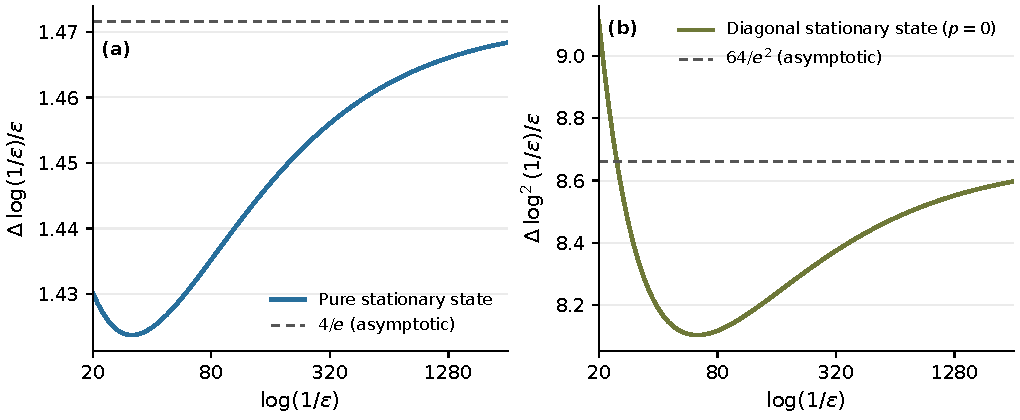
\includegraphics[width=\columnwidth]{reset_convergence.pdf}
 \caption{显式可实现的重置构造，其中实际增益为 $\Delta=\eps-a$，实际输出误差为 $\eps=P(0|1)$。（a）纯稳态族 \eqref{eq:familyparams}--\eqref{eq:familyjump} 经对数缩放后趋于 $4/e$。（b）满足 $p=0$ 的对角稳态族 \eqref{eq:diag-jump}--\eqref{eq:diag-xstar} 经 $\log^2(1/\eps)$ 缩放后趋于 $64/e^2$。实线由上述显式生成元计算得到，虚线表示渐近常数。}
 \label{fig:convergence}
\end{figure}


\section{与四参数族的关系}\label{app:prior-family}

文献 \cite{Shahbeigi2024} 中用于数值搜索边界的族满足
\begin{equation}\label{eq:prior-family}
 \begin{gathered}
 H_{\rm old}=X,\\
 J_{\rm old}=\sqrt\gamma\,\ket{\psi_o}\bra{\psi_i},\\
 \ket{\psi_j}=\binom{\cos\theta_j}{i\sin\theta_j},
 \\ \gamma,t>0.
 \end{gathered}
\end{equation}
该族的参数没有物理上界。搜索中采用的数值容差并不限制这一数学族。

对纯稳态构造的每组固定有限参数，有
\begin{equation}\label{eq:prior-pure-rankone}
 J=\sqrt{A+B}\ket u\bra e,\qquad
 \ket u=\frac{-\sqrt B\ket e+\sqrt A\ket g}{\sqrt{A+B}}.
\end{equation}
向量 $u,e$ 在测量基中为实。酉算符 $S=\diag(1,i)$ 保持制备和测量投影算符不变，并将任意归一化实向量变为式 \eqref{eq:prior-family} 的形式。令 $V_{\rm old}=S\ket u\bra eS^\dagger$。当 $t_n\downarrow0$ 且 $\gamma_nt_n=A+B$ 时，原有族中的信道满足
\begin{equation}\label{eq:prior-pure-limit}
 \exp\!\left(-it_n[X,\cdot]+(A+B)\Diss[V_{\rm old}]\right)
 \longrightarrow \exp\!\left(\Diss[SJS^\dagger]\right).
\end{equation}
由有限维矩阵指数的连续性，每个这样的转移表都属于原有族的概率闭包。此逼近是在固定 $A,B,p$ 时进行的；随后再取独立极限 $L\to\infty$，趋近重置。

对于式 \eqref{eq:diag-jump} 中的对角构造，当 $\nu$ 足够小时，有 $\tau=2/\log(1/\nu)>4\chi$。此时实跳跃矩阵具有负实特征值 $\xi$，满足
\begin{equation}\label{eq:prior-diag-shift}
 \begin{gathered}
 \xi^2+\sqrt B\,\xi+A\chi=0,\\
 J'=J-\xi I,\\
 H'=H+\frac{i\xi}{2}(J-J^\dagger).
 \end{gathered}
\end{equation}
这一恒等分量平移保持 GKSL 生成元不变。由于 $J'$ 非零、为实且奇异，其秩为一。此外，
\begin{equation}\label{eq:prior-diag-hamiltonian}
 \begin{gathered}
 H'_{12}=ik',\\
 k'=\kappa_H-\frac{\xi}{2}(\sqrt A+\sqrt U)>0,\\
 SH'S^\dagger=k'X.
 \end{gathered}
\end{equation}
写为 $J'=s\ket{u'}\bra{v'}$，其中 $s>0$，两个向量为实单位向量。在同一相位变换之后，选取原有族的持续时间 $t=k'$ 和跳跃速率 $\gamma=s^2/k'$。其累积生成元恰好等于对角构造经变换后的时间一生成元。因此，对所有充分小的 $\nu$，该族就属于原有四参数族本身。

这些变换确立了上述构造与已有四参数族之间的关系。

\section{排除区域的比较}\label{app:exclusions}\label{sec:exclusions}

为与已有解析排除界比较，记文献 \cite{Shahbeigi2024} 定理 1 中重置一侧的函数为
\begin{equation}\label{eq:oldg}
 g_R(a)=(2-a)(2a+a^{1/10}).
\end{equation}
该定理排除满足 $a\le10^{-6}$、$\eps>g_R(a)$，以及另一个将转移表与交换端点区分开的条件的转移表。在重置附近，第二个条件自动成立。由于
$g_R(a)=2a^{1/10}[1+o(1)]$ 局部递增，对其反演可得必要下界
\begin{equation}\label{eq:oldinverse}
 a\ge(\eps/2)^{10}[1+o(1)].
\end{equation}
这是由已有界导出的比较结果，不是真实边界的渐近公式。

为了直接比较开区域，固定 $C>4/e$，并选择 $\eps_C>0$，使定理 \ref{thm:main} 在该阈值以下给出 $a\ge\eps[1-C/\log(1/\eps)]$。集合
\begin{equation}\label{eq:newwedge}
 \begin{split}
 \mathcal W_C=\bigl\{(a,1-\eps):\;&0<\eps<
 \min(\eps_C,e^{-4C},10^{-6}),\\
 &\eps/2<a<3\eps/4\bigr\}
 \end{split}
\end{equation}
中的每个转移表都被本文的界排除，却均不能被已有定理或其交换坐标后的版本排除。事实上，对 $0<a<1$，有
$g_R(a)>2a(2-a)>2a>\eps$，因此原有重置条件不成立；交换坐标后，第一个坐标接近一，也不满足其小坐标前提。所以这一改进覆盖非零面积，无需借助数值边界估计。

\begin{thebibliography}{5}
\bibitem{Shahbeigi2024}
F.~Shahbeigi, C.~T.~Chubb, R.~Kukulski, {\L}.~Pawela, and K.~Korzekwa,
Quantum-embeddable stochastic matrices,
\href{https://doi.org/10.22331/q-2024-07-10-1404}{\emph{Quantum} \textbf{8}, 1404 (2024)}.

\bibitem{KorzekwaLostaglio2021}
K.~Korzekwa and M.~Lostaglio,
Quantum advantage in simulating stochastic processes,
\href{https://doi.org/10.1103/PhysRevX.11.021019}{\emph{Phys. Rev. X} \textbf{11}, 021019 (2021)}.

\bibitem{Benatti2024}
F.~Benatti, D.~Chru\'sci\'nski, and G.~Nichele,
Quantum versus classical $P$-divisibility,
\href{https://doi.org/10.1103/PhysRevA.110.052212}{\emph{Phys. Rev. A} \textbf{110}, 052212 (2024)}.

\bibitem{GKS1976}
V.~Gorini, A.~Kossakowski, and E.~C.~G.~Sudarshan,
Completely positive dynamical semigroups of $N$-level systems,
\href{https://doi.org/10.1063/1.522979}{\emph{J. Math. Phys.} \textbf{17}, 821--825 (1976)}.

\bibitem{Lindblad1976}
G.~Lindblad,
On the generators of quantum dynamical semigroups,
\href{https://doi.org/10.1007/BF01608499}{\emph{Commun. Math. Phys.} \textbf{48}, 119--130 (1976)}.

\end{thebibliography}
\end{document}



